
\documentclass[10pt]{article}
\usepackage[margin=0.75in]{geometry}
\usepackage{graphicx}
\usepackage{booktabs}
\usepackage{caption}
\usepackage{xcolor}
\usepackage{hyperref}
\usepackage{amsmath}
\title{O1 Baseline Comparison on the Fixed 474-GM Test Set}
\author{Seismic-FNO Internal Report}
\date{June 2026}
\begin{document}
\maketitle
\section*{Protocol}
Full-data O1 comparison on the canonical fixed split: 2,400 train ground motions, 600 validation ground motions, and 474 held-out test ground motions. All models use batch size 64 and 50 epochs. Reported metrics are measured on the fixed 474-GM test set.
\section*{Executive Summary}
\begin{itemize}
  \item BiLSTM achieved the lowest test MSE (0.0099) and highest R2 (0.9872), but required the longest training time (7.51 h) and largest memory footprint (15.61 GB).
  \item The stabilized pre-norm Transformer ranked second in MSE (0.0214) with substantially lower memory than BiLSTM (2.54 GB).
  \item FNO-Large was resource efficient but underperformed BiLSTM/Transformer on this O1 fixed 474-GM test split (MSE 0.0449).
  \item The original Transformer run collapsed to a mean-prediction regime and was excluded after replacing it with a standard pre-norm Transformer and a lower learning rate.

\end{itemize}
\section*{Quantitative Results}
\begin{table}[h]
\centering
\small
\caption{Fixed 474-GM test accuracy and resource costs.}
\begin{tabular}{lrrrrrrrr}
\toprule
Model & MSE $\downarrow$ & $R^2$ $\uparrow$ & PFA RMSE $\downarrow$ & Spec $\downarrow$ & High-f $\downarrow$ & Train h $\downarrow$ & GPU GB $\downarrow$ & Lat. ms $\downarrow$ \\
\midrule
BiLSTM & 0.0099 & 0.9872 & 0.0182 & 0.185 & 0.222 & 7.51 & 15.61 & 1.049 \\
Transformer & 0.0214 & 0.9725 & 0.0231 & 0.325 & 0.391 & 2.34 & 2.54 & 0.106 \\
FNO-Large & 0.0449 & 0.9423 & 0.0330 & 0.342 & 0.398 & 2.16 & 3.30 & 0.108 \\
ResCNN1D & 0.1481 & 0.8096 & 0.0547 & 0.484 & 0.534 & 6.29 & 3.49 & 0.607 \\
UNet1D & 0.2157 & 0.7227 & 0.1063 & 0.588 & 0.633 & 2.27 & 3.03 & 0.096 \\
MLP & 0.7420 & 0.0462 & 0.2464 & 1.255 & 1.091 & 1.59 & 0.24 & 0.075 \\
\bottomrule
\end{tabular}
\end{table}
\begin{figure}[h]
\centering
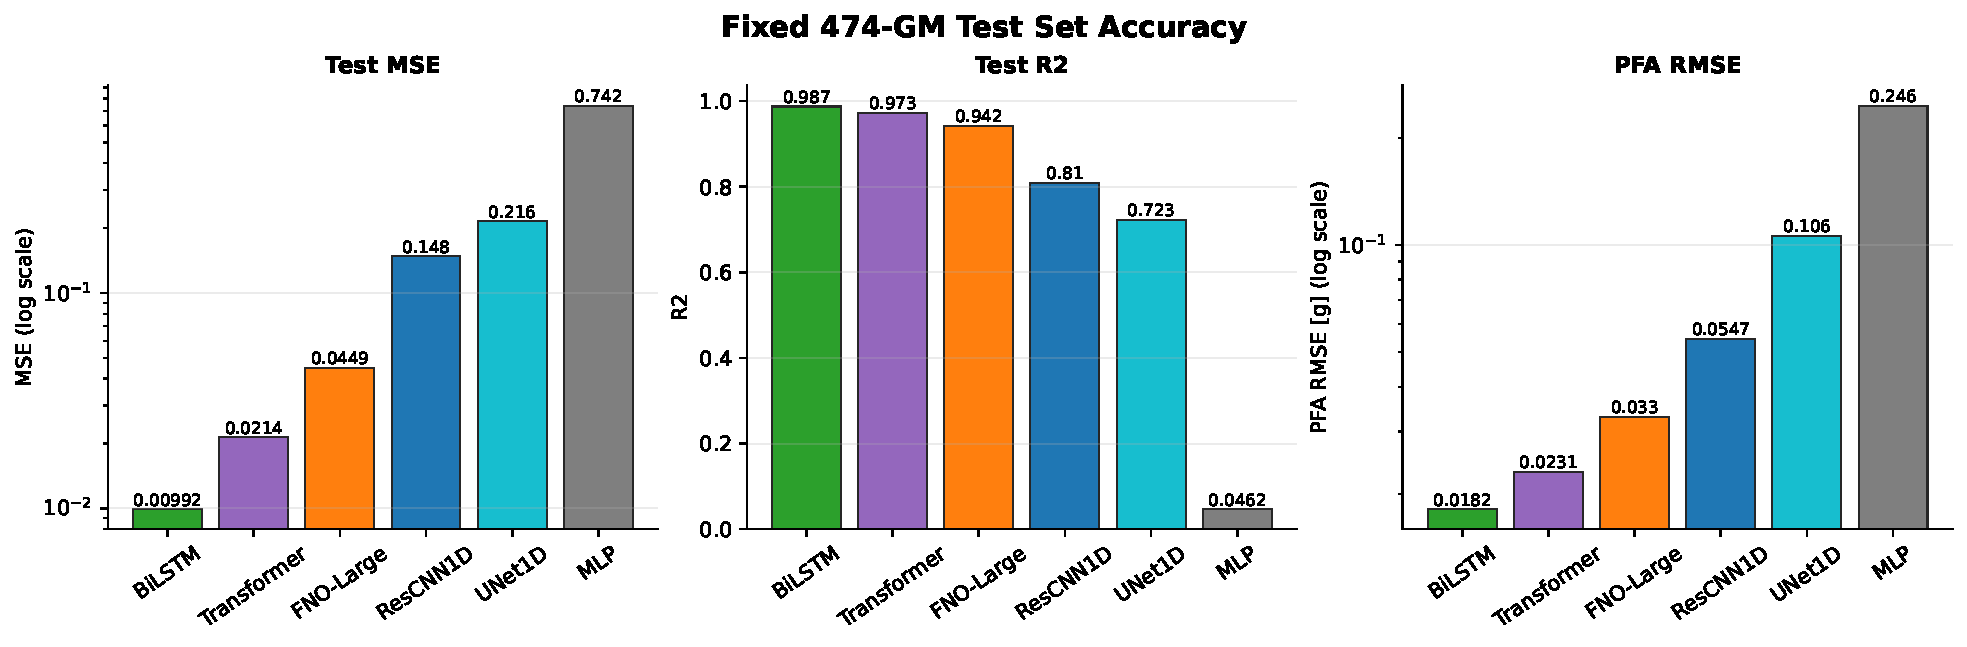
\includegraphics[width=0.98\linewidth]{figures/fig1_test_accuracy.pdf}
\caption{Main test-set accuracy metrics.}
\end{figure}
\begin{figure}[h]
\centering
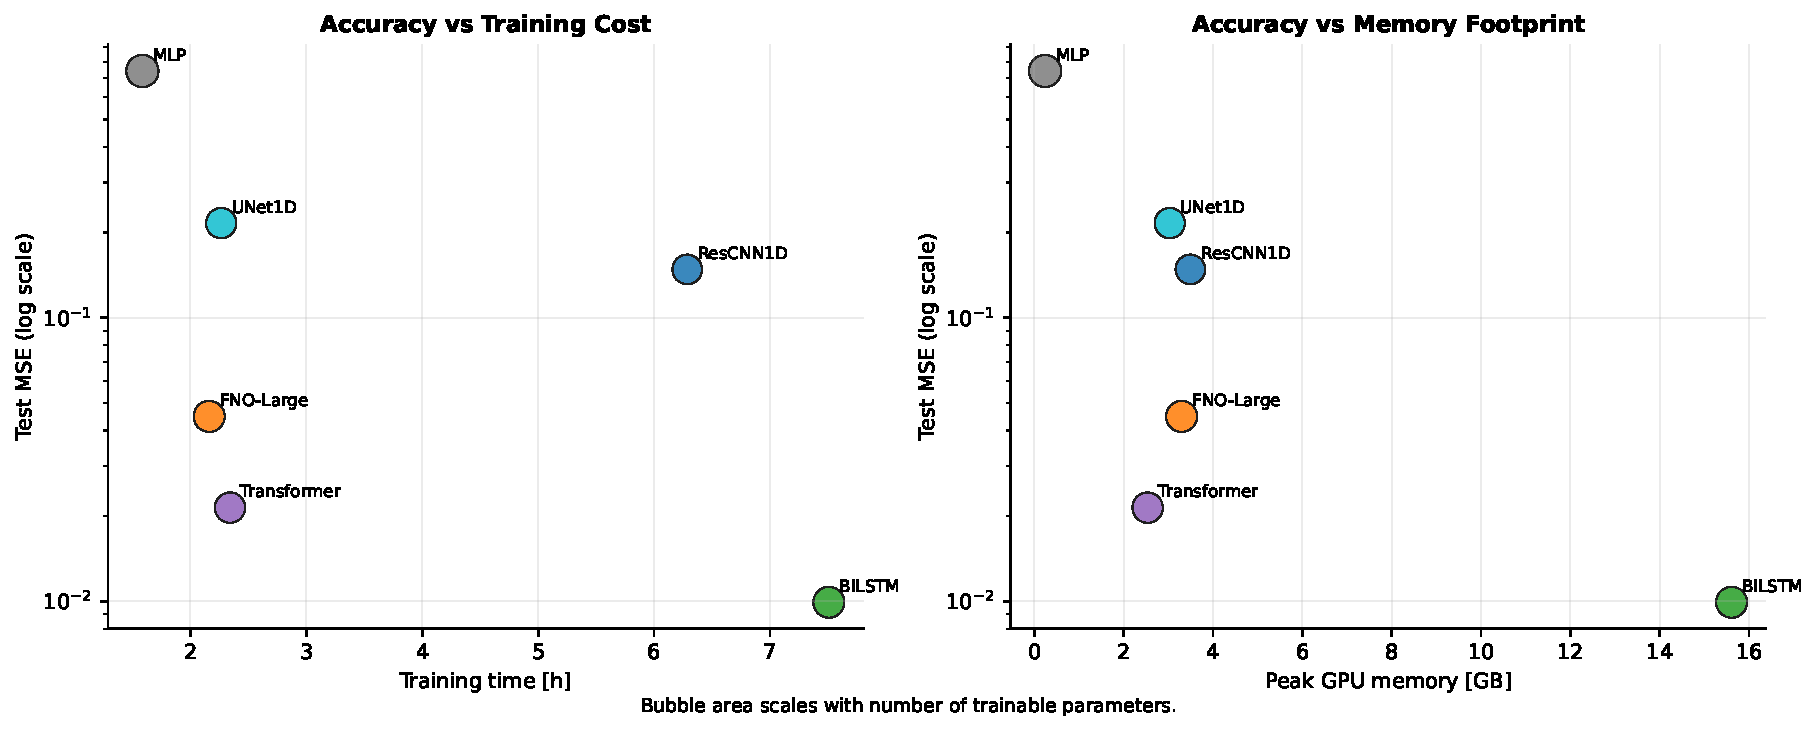
\includegraphics[width=0.98\linewidth]{figures/fig2_tradeoff_bubbles.pdf}
\caption{Accuracy-resource tradeoffs. Bubble area scales with parameter count.}
\end{figure}
\begin{figure}[h]
\centering
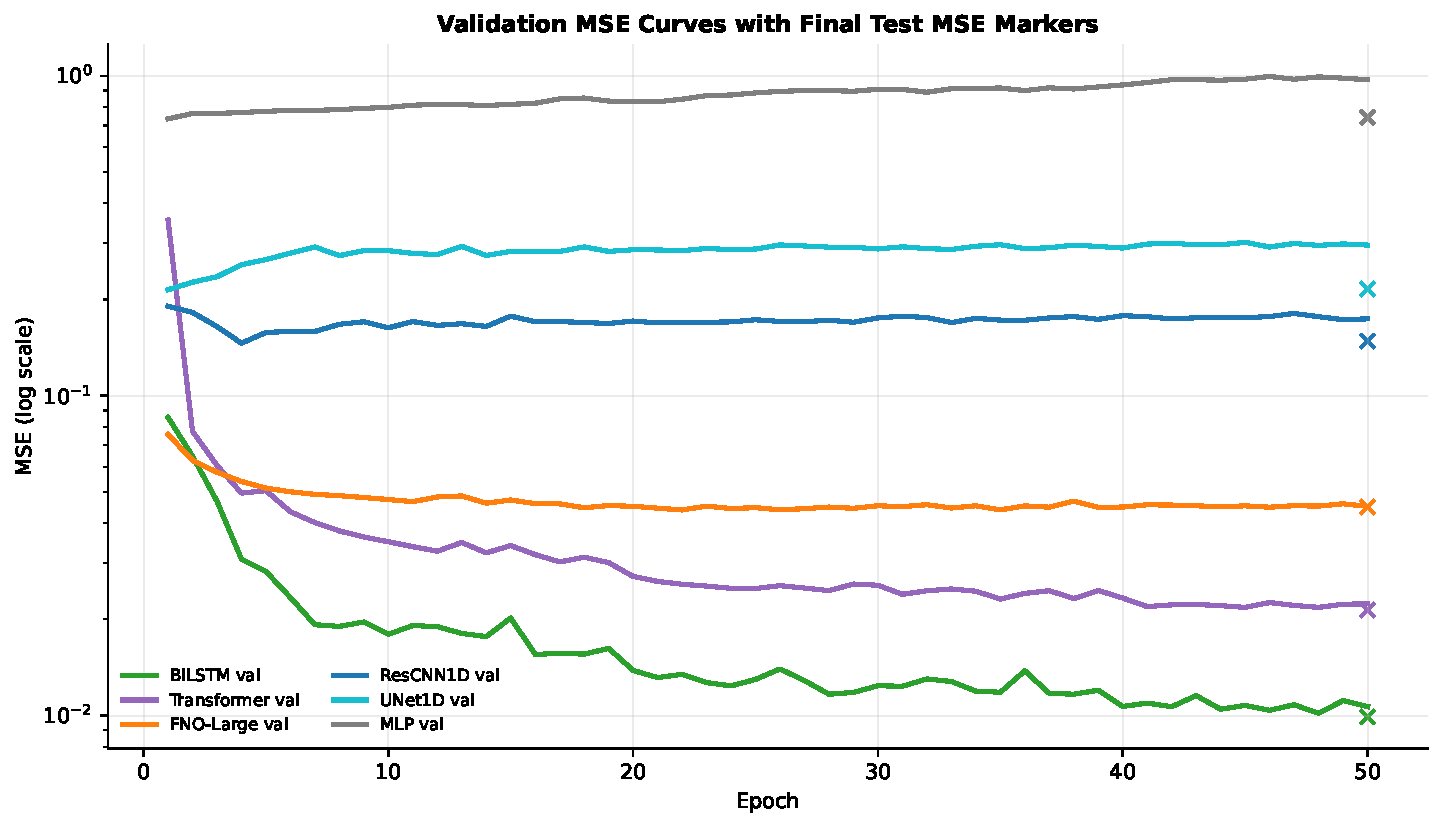
\includegraphics[width=0.98\linewidth]{figures/fig3_training_curves.pdf}
\caption{Validation MSE curves with final test MSE markers.}
\end{figure}
\begin{figure}[h]
\centering
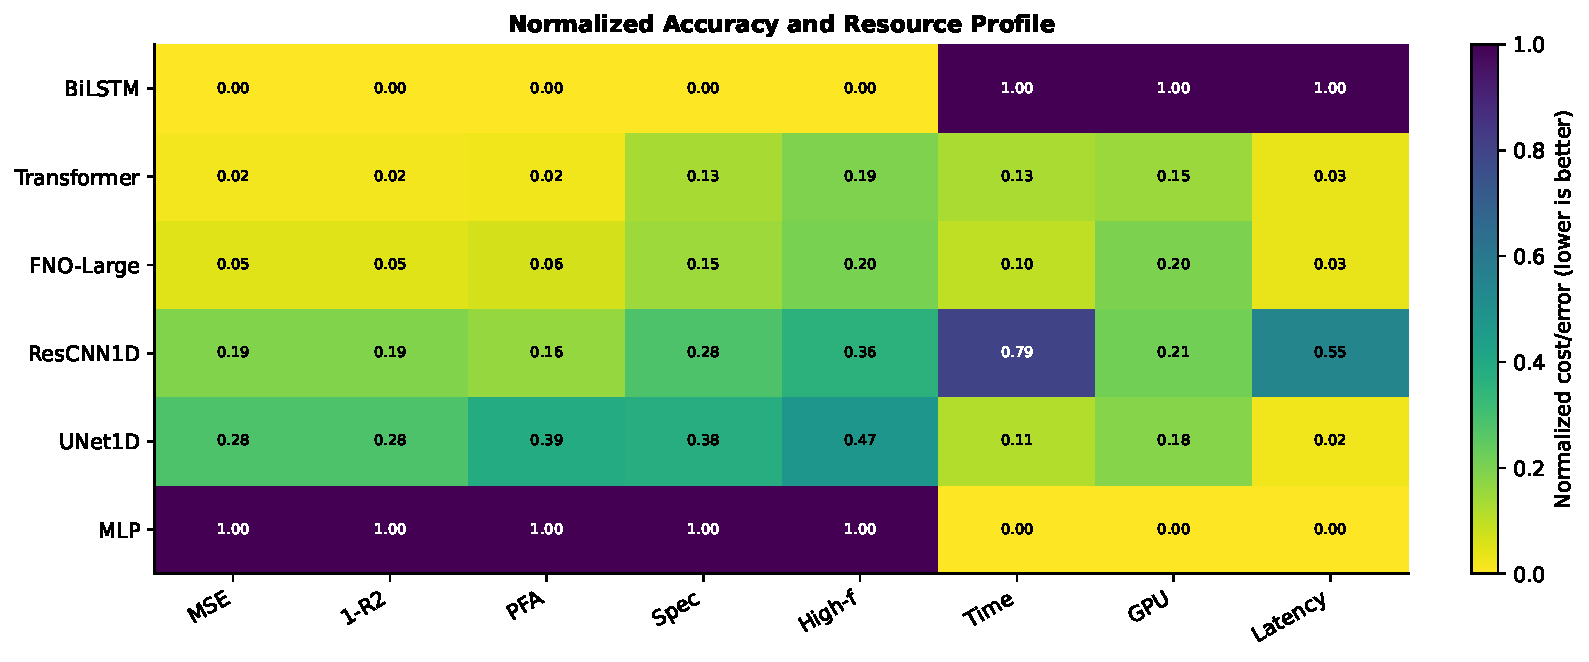
\includegraphics[width=0.98\linewidth]{figures/fig4_normalized_profile.pdf}
\caption{Normalized error and cost profile. Lower is better for all columns.}
\end{figure}
\section*{Interpretation}
BiLSTM is the strongest model in raw test accuracy, but it is also the most expensive model to train and deploy in memory. The stabilized pre-norm Transformer is a strong second and provides a better memory/latency tradeoff. FNO-Large remains competitive and resource efficient, but it does not dominate this particular in-distribution fixed-test protocol. OOD and classical-GM experiments should be used to assess whether FNO has advantages outside the i.i.d. split.
\end{document}
